\documentclass{beamer}
\usetheme{Boadilla}
\setbeamertemplate{caption}[numbered]

\usepackage{natbib}
\usepackage{xcolor}
\usepackage{booktabs}
\usepackage{appendixnumberbeamer}
\bibliographystyle{apalike}

\newcommand{\red}[1]{\textcolor{red}{#1}}
\newcommand{\blue}[1]{\textcolor{blue}{#1}}

\defcitealias{myers1984corporate}{MM84}
\defcitealias{gertner1994internal}{GSS94}
\defcitealias{holmstrom1998private}{HT98}
\defcitealias{brunnermeier2009market}{BP09}
\defcitealias{he2013intermediary}{HK13}
\defcitealias{diamond1983bank}{DD83}
\defcitealias{diamond1984financial}{D84}
\defcitealias{gorton1990financial}{GP90}
\defcitealias{hanson2015banks}{HSSV15}
\defcitealias{kashyap2002banks}{KRS02}
\defcitealias{holmstrom1997financial}{HT97}
\defcitealias{bolton2011outside}{BSS11}

\title[Youth and redistribution]{Why do young Americans support redistribution?}
\subtitle{Survey evidence on a widening U.S. age gap}
% Documenting a widening U.S. age gap and its drivers

\author[Carlson and Rancière]{Niclas Carlson and Romain Rancière}
% \institute{Columbia Business School}
\date{\today}

\begin{document}


\begin{frame}
\titlepage
\end{frame}



\begin{frame}{Summary}
\begin{enumerate}
    \item The US young-old gap in support for redistribution went from zero in the 1970s–80s to +0.5 SD today (half of the party gap, similar to the race gap, double the gender gap).
    \item It is not the economic position of the young: 26 measures of income, risk and prospects explain none of the gap.
    \item It is what the young believe about the economy: zero-sum and attribution beliefs account for a half to four-fifths of the gap.
    \item Ongoing analysis: what drives these beliefs?
\end{enumerate}
\end{frame}



\begin{frame}{The 2025 Prolific survey}
\begin{itemize}
    \item Purpose-built online survey of U.S. adults, fielded on Prolific in 2025.
    \item $N \approx 2{,}000$, sampled to be balanced around age 30 (half younger, half older) to power the young--old comparison.
    \item Three redistribution outcomes: government should reduce income differences, federal tax progressivity, and support for a revenue-neutral tax-shift proposal.
    \item Built to test the two hypotheses head-to-head: 26 self-interest constructs (income, financial position, long-term risk, upward-mobility prospects, time preference) against beliefs and values (zero-sum, attribution/deservingness, fairness).
    \item Benchmarked against external surveys: \cite{chinoy2026zero}, GSS, ANES, and WVS/EVS.
\end{itemize}
\end{frame}



\begin{frame}{Motivation}

\begin{figure}
    \centering
    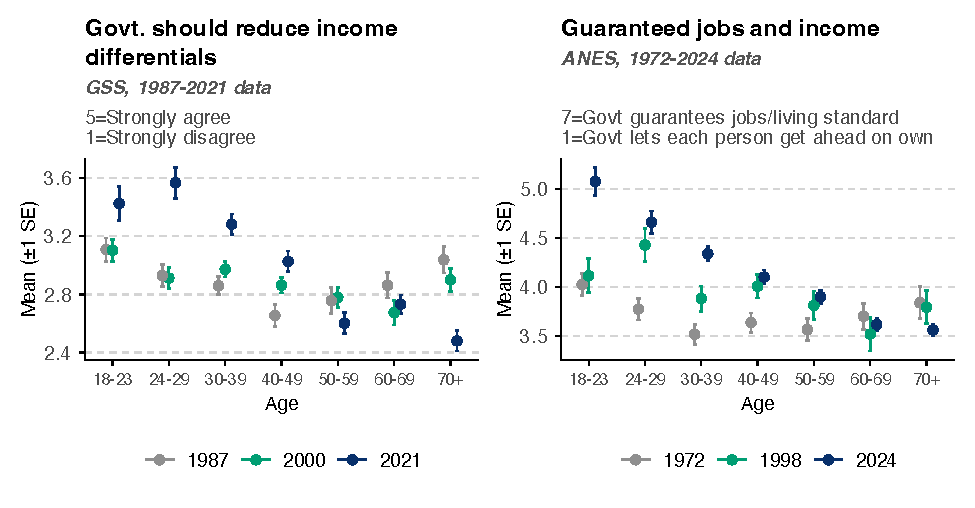
\includegraphics[width=0.9\linewidth]{figures/fig_slide_profile_pair.pdf}
    \label{fig:placeholder}
    \caption{Cross-sectional age gradient steepening over time}
\end{figure}
    
\end{frame}



\begin{frame}{Motivation}

\begin{figure}
    \centering
    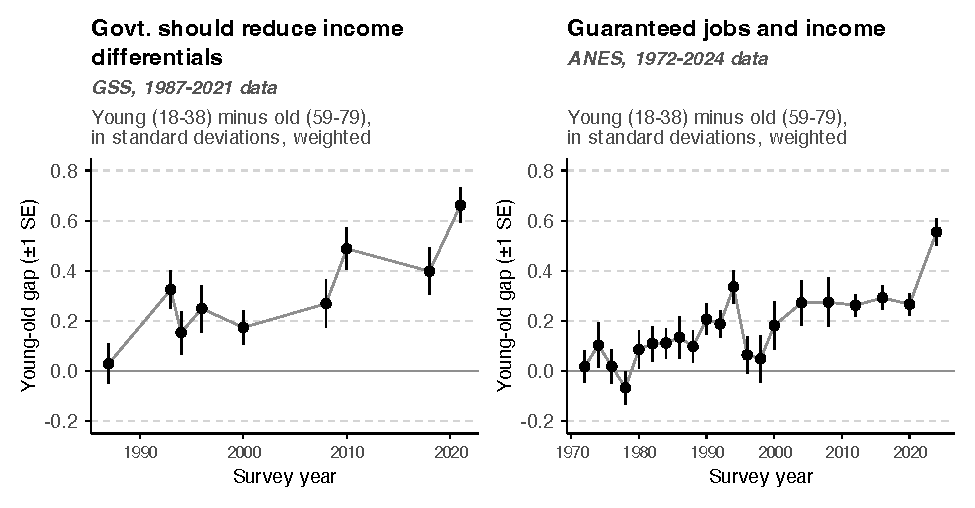
\includegraphics[width=0.9\linewidth]{figures/fig_slide_gap_pair.pdf}
    \label{fig:placeholder}
    \caption{Young-old age gap increasing over time}
\end{figure}
    
\end{frame}



\begin{frame}{Motivation}
% Redistribution, not just support

\begin{figure}
    \centering
    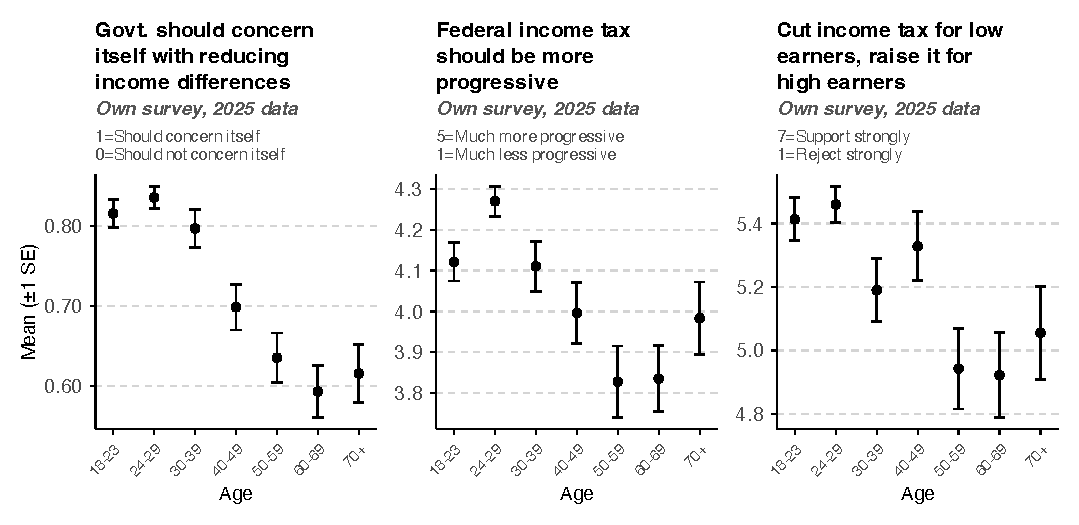
\includegraphics[width=0.95\linewidth]{figures/fig_slide_prolific_triple.pdf}
    \label{fig:placeholder}
    \caption{Current age gap on tax redistribution}
    % Cross-sectional age gradient in 2025 Prolific online survey
\end{figure}
    
\end{frame}



\begin{frame}{Age or cohort effects?}

Two competing hypotheses: 
\begin{itemize}
    \item Lifecycle: currently low  income + time discounting, present stress, long-term career/financial risk, prospect of upward mobility. 
    
    \vspace{0.2em}
    Largely \textit{self-interest}-driven.
    \item Cohort divergence: inequality, growth, mobility, housing prices, social safety net access, diversity, immigration. Shaped by political narratives and the supply of politicians/platforms.
    % (who to blame) (electoral institutions)

    \vspace{0.2em}
    Largely \textit{belief}-driven.
    % Real economic conditions 
\end{itemize}
    
\end{frame}



\begin{frame}{Lifecycle self-interest explains little}

\begin{figure}
    \centering
    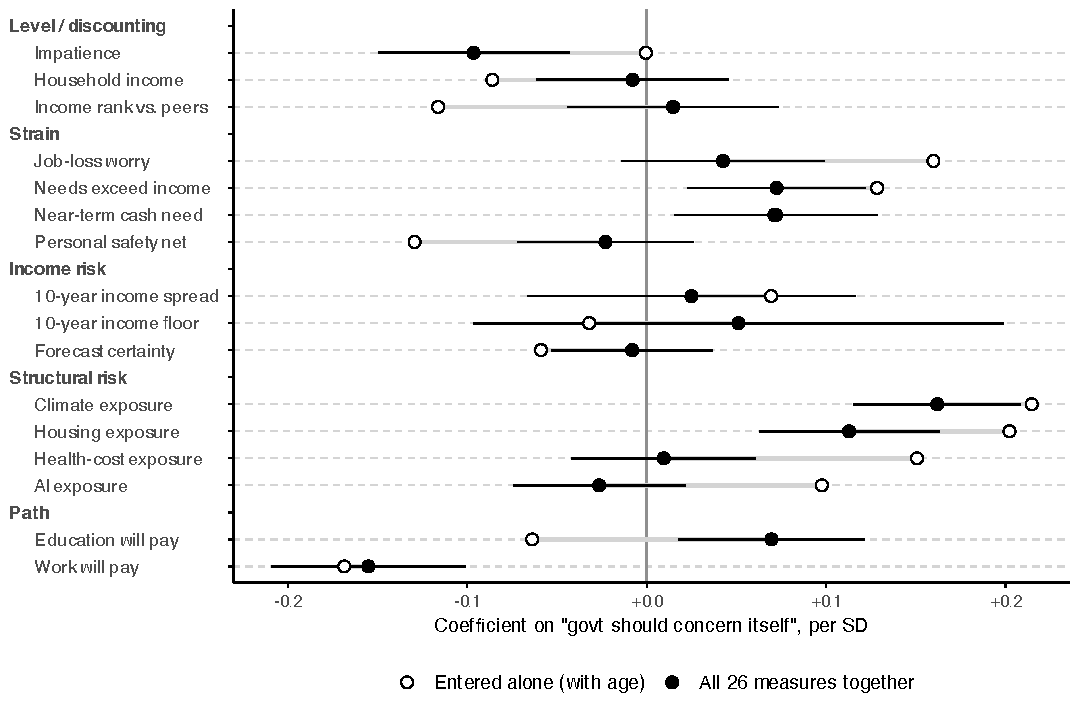
\includegraphics[width=0.8\linewidth]{figures/fig_slide_alone_vs_together.pdf}
    \caption{\centering Redistributive preferences vs. 26 self-interest constructs. \newline Including all variables, $R^2$ is only $0.11$.}
    \label{fig:placeholder}
\end{figure}
% Beliefs about the economy explain 24-45\%.
    
\end{frame}



\begin{frame}{Lifecycle self-interest explains little}

Decomposing the age gradient, long-term risk and prospect of upward mobility push youth in opposite directions.
\begin{figure}
    \centering
    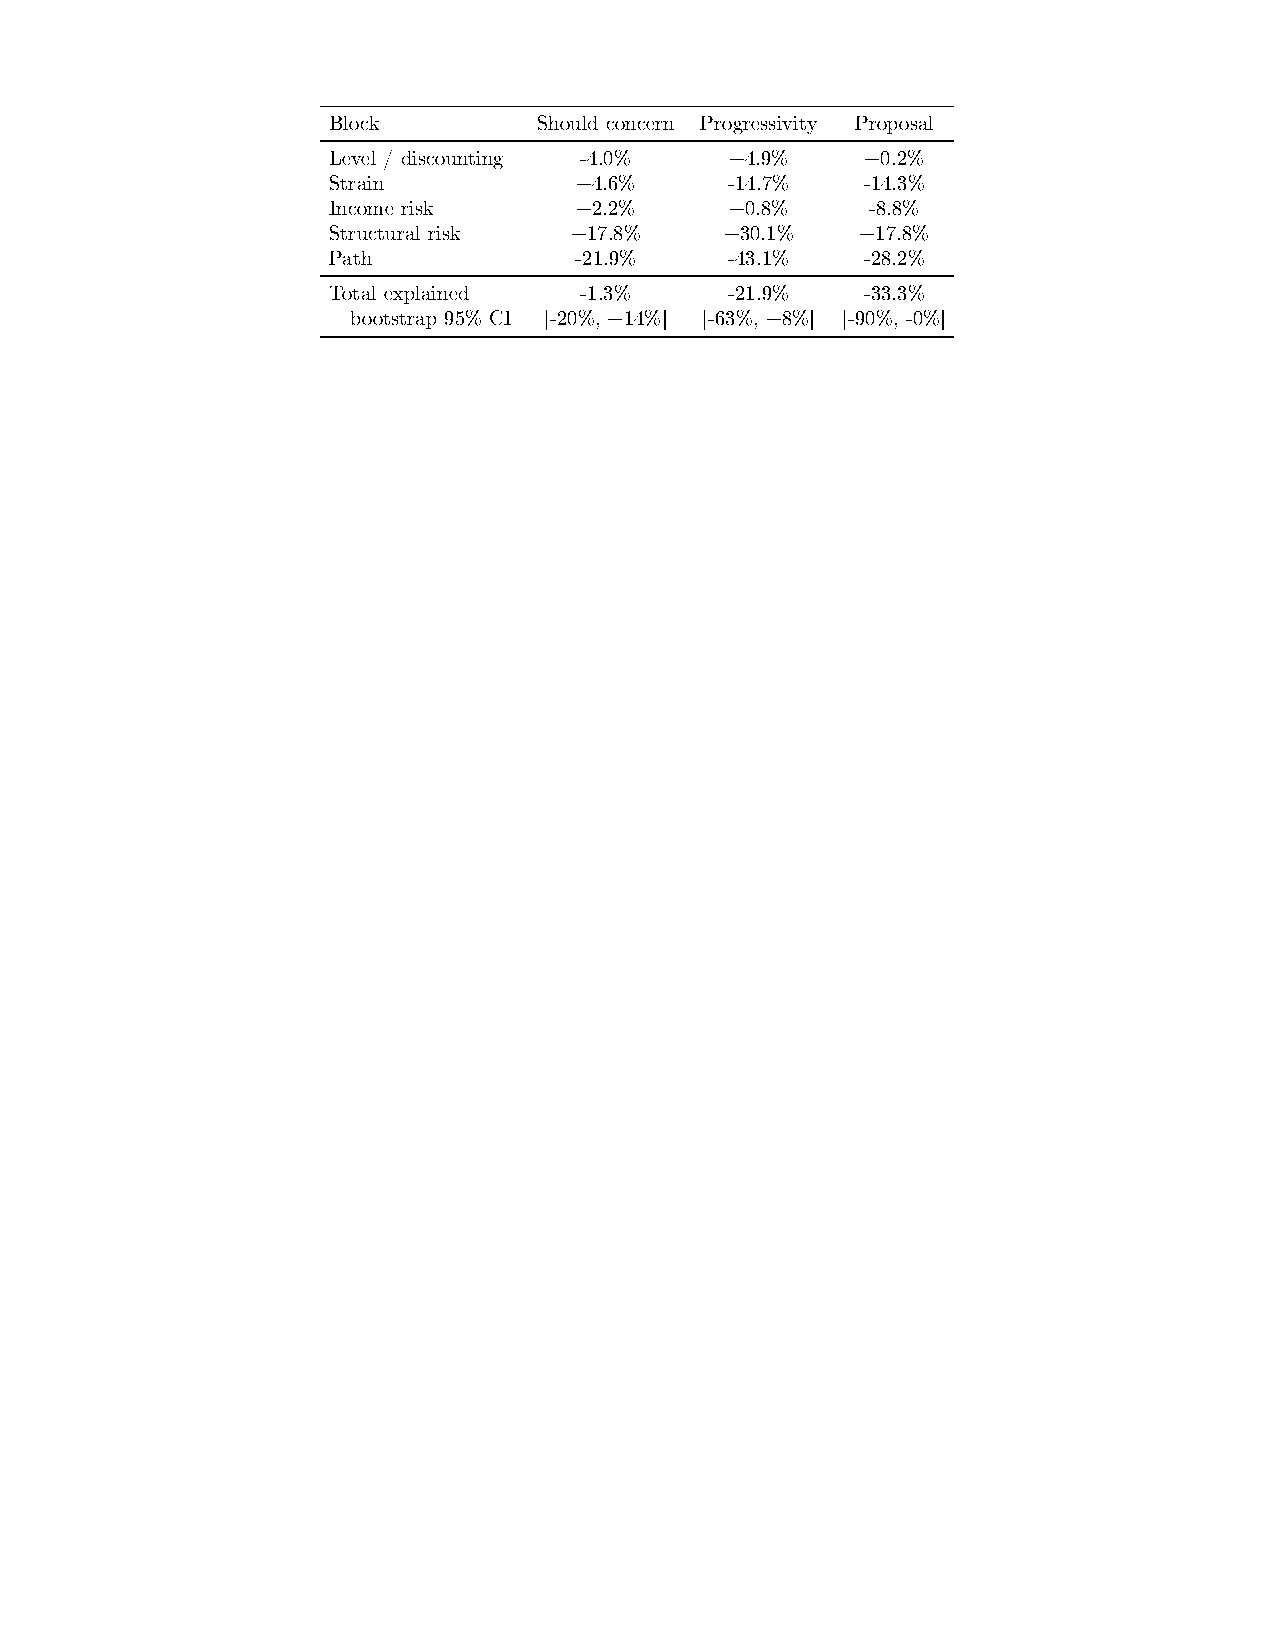
\includegraphics[width=0.8\linewidth]{figures/table_gelbach_slide.pdf}
    \caption{Gelbach decomposition of age-redistribution slope}
    \label{fig:placeholder}
\end{figure}

    
\end{frame}



\begin{frame}{Testing channels head-to-head}
% Testing both channels

\begin{figure}
    \centering
    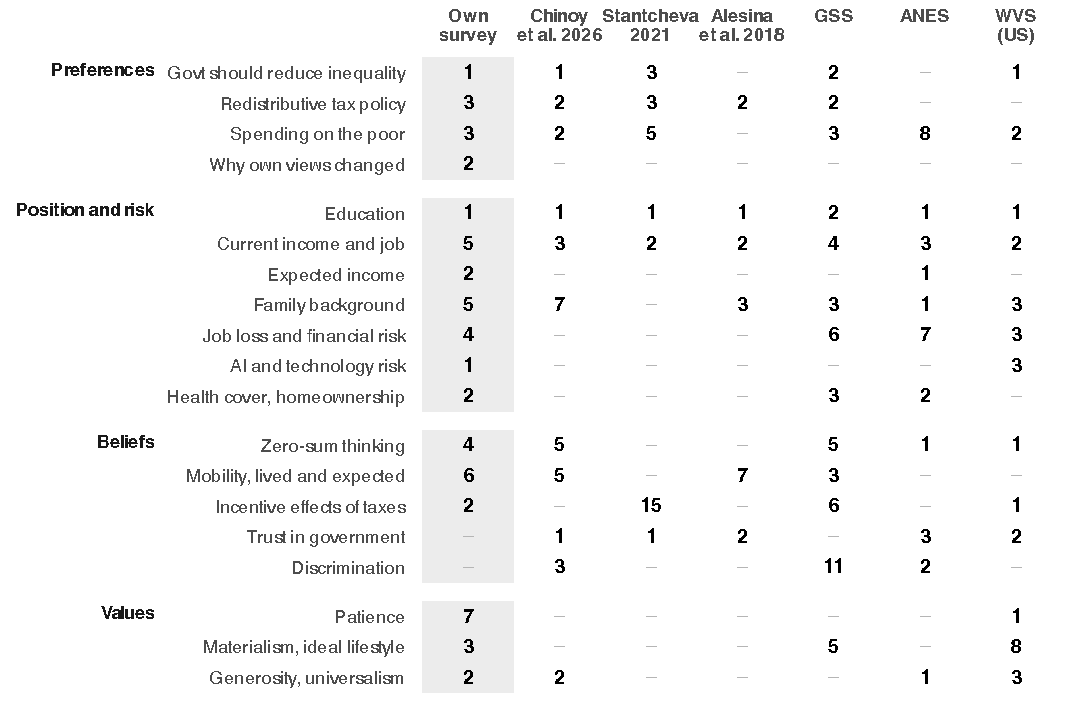
\includegraphics[width=0.85\linewidth]{figures/fig_slide_coverage.pdf}
    \caption{Mechanisms covered in 2025 Prolific online survey}
    \label{fig:placeholder}
\end{figure}

    
\end{frame}



\begin{frame}{Correlates of redistributive preferences}
% What drives preferences for redistribution?

% Head-to-head, are economic position, demographics, beliefs, or values most correlated?
\begin{figure}
    \centering
    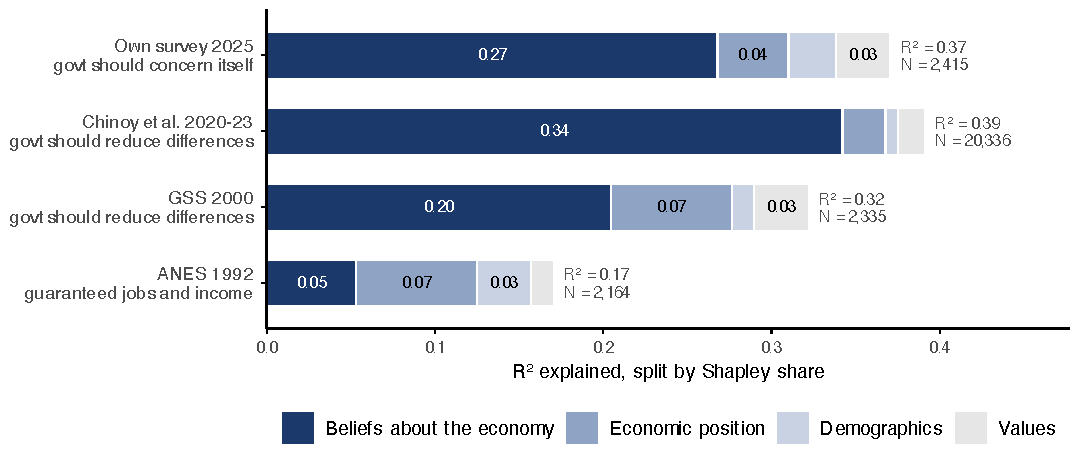
\includegraphics[width=0.9\linewidth]{figures/fig_slide_shapley_groups.pdf}
    \caption{Shapley $R^2$ decomposition of redistributive preferences}
\end{figure}
    
\end{frame}



\begin{frame}{Correlates of redistributive preferences}

\begin{figure}
    \centering
    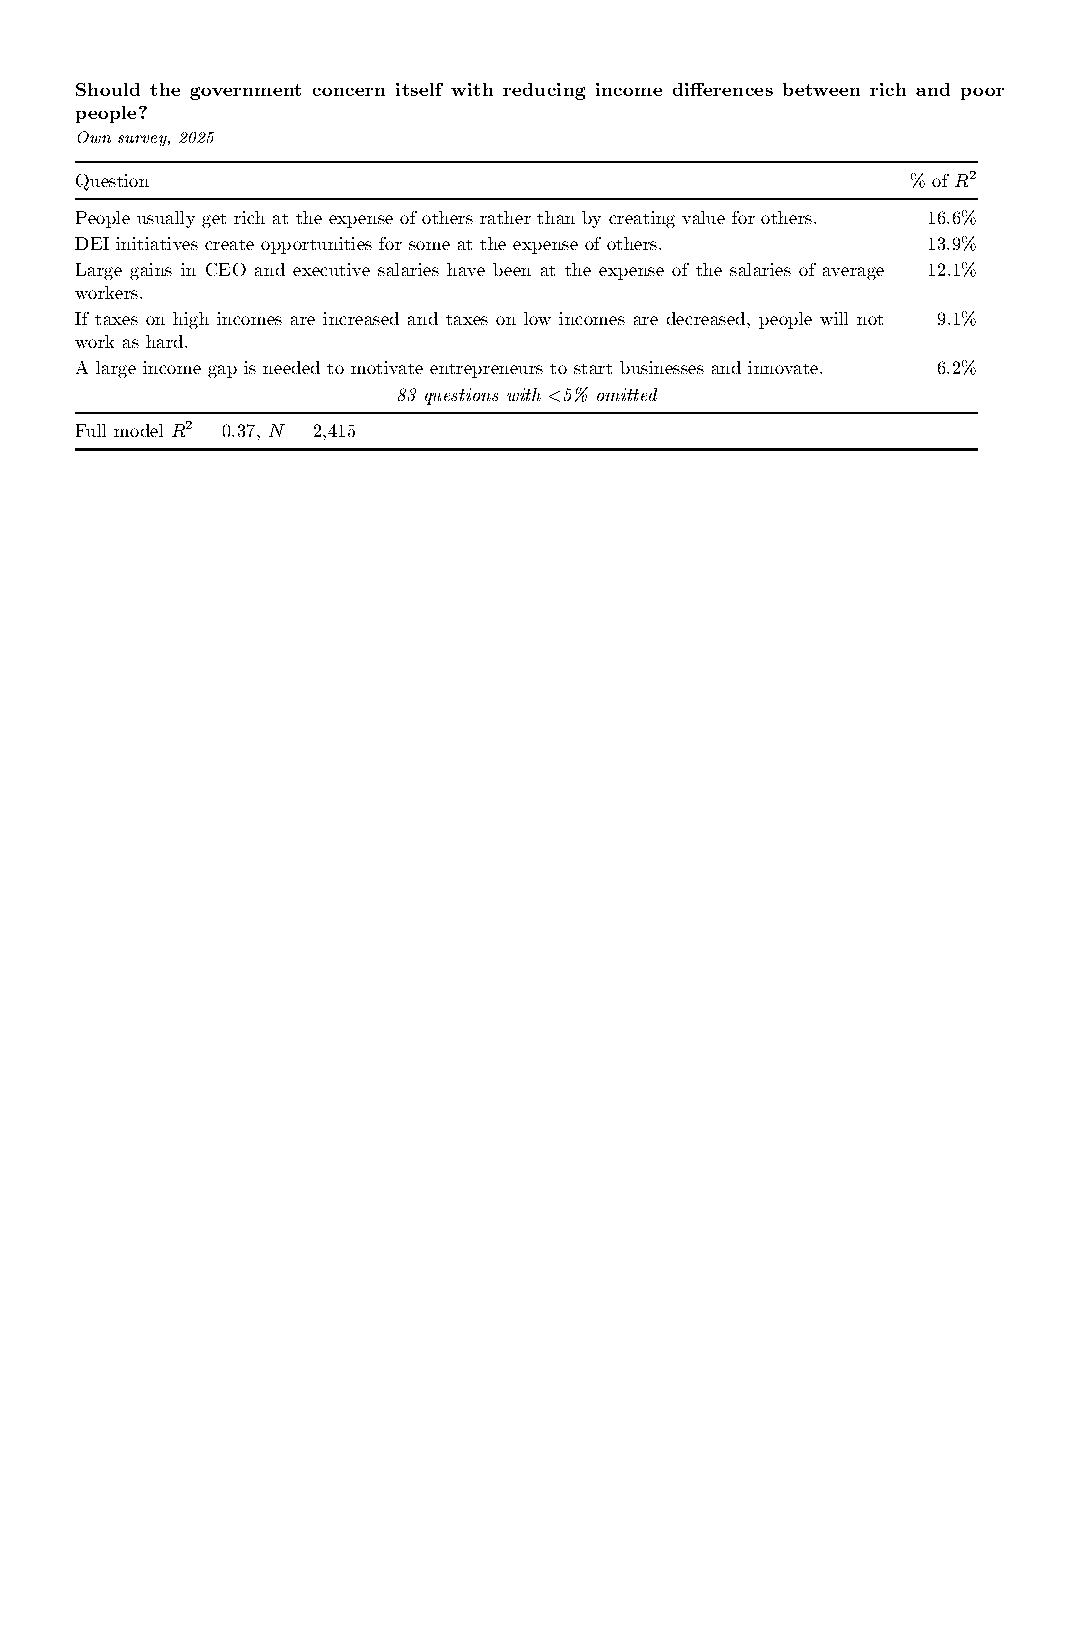
\includegraphics[width=0.9\linewidth]{figures/table_slide_shapley_own.pdf}
    \caption{Shapley $R^2$ decomposition of 2025 Prolific survey}
    \label{fig:placeholder}
\end{figure}
    
\end{frame}



\begin{frame}{Correlates of redistributive preferences}

\begin{figure}
    \centering
    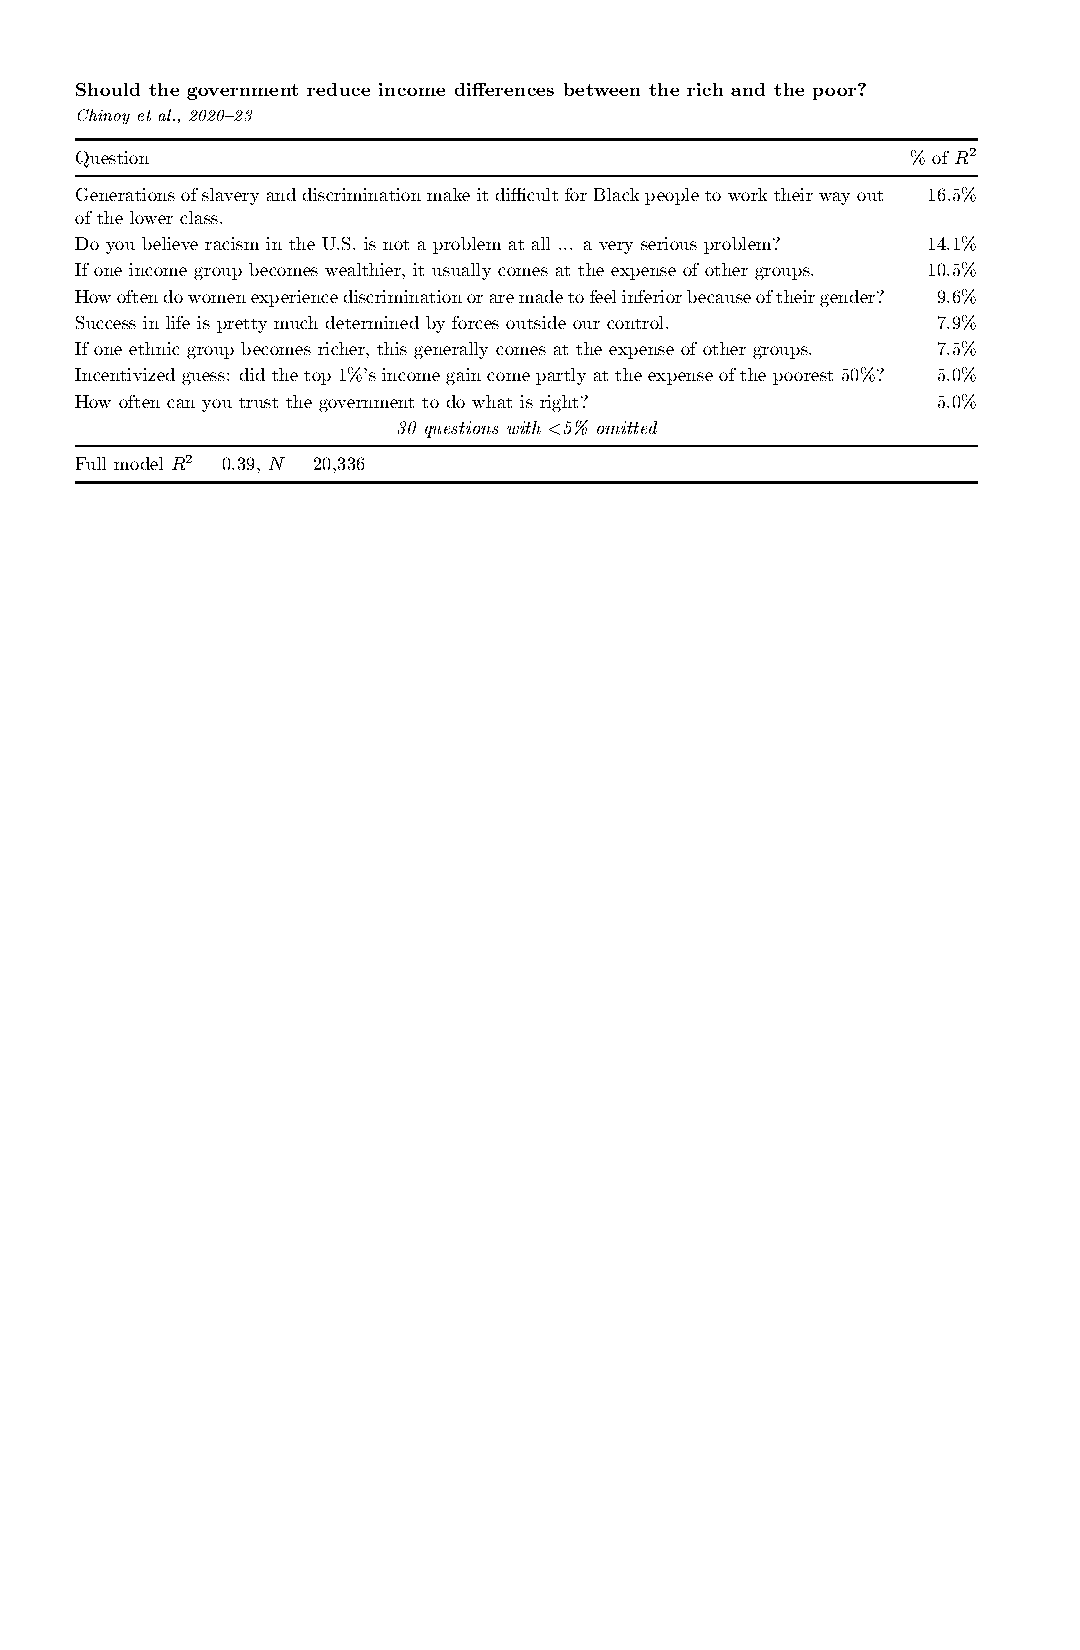
\includegraphics[width=0.9\linewidth]{figures/table_slide_shapley_chinoy.pdf}
    \caption{Shapley $R^2$ decomposition of \cite{chinoy2026zero}}
    \label{fig:placeholder}
\end{figure}
    
\end{frame}



\begin{frame}{Decomposing the age gradient}

\begin{figure}
    \centering
    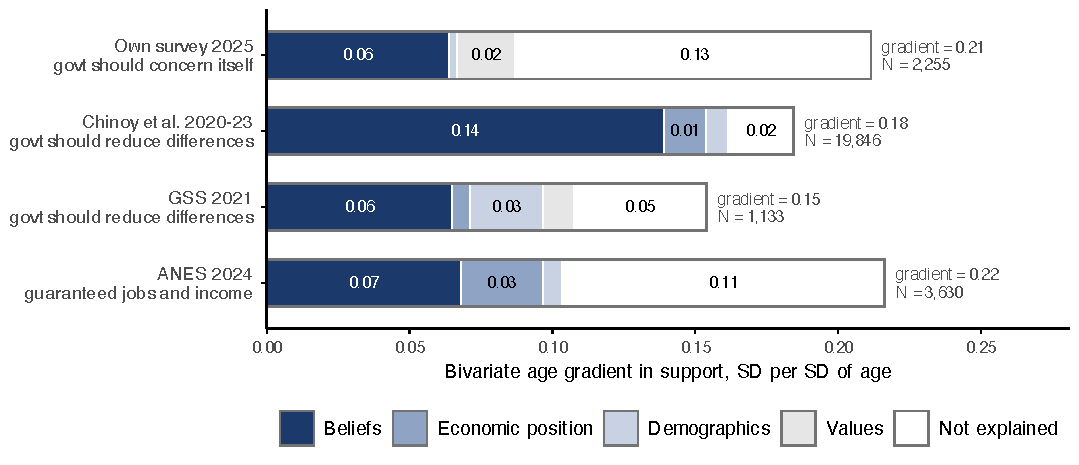
\includegraphics[width=0.9\linewidth]{figures/fig_slide_gelbach_groups.pdf}
    \caption{Gelbach decomposition of age-redistribution slope}
    \label{fig:placeholder}
\end{figure}
    
\end{frame}



\begin{frame}{Decomposing the age gradient}

\begin{figure}
    \centering
    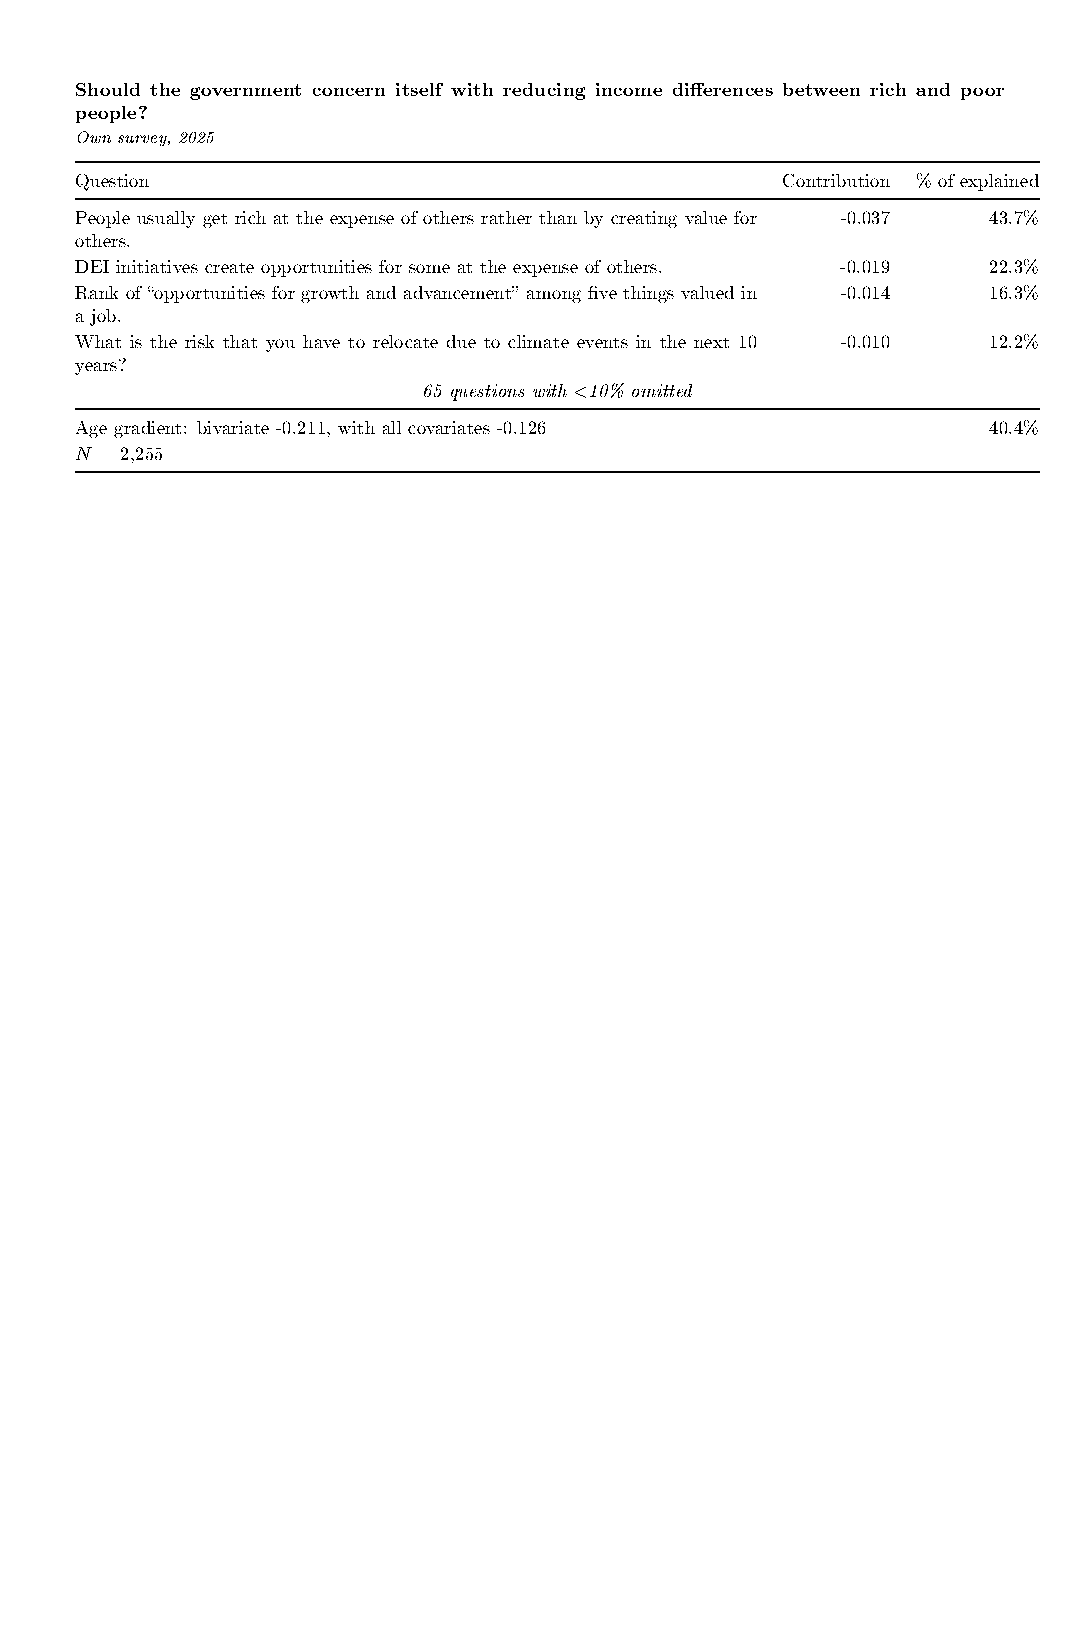
\includegraphics[width=0.9\linewidth]{figures/table_slide_gelbach_own.pdf}
    \caption{Gelbach decomposition of 2025 Prolific survey}
    \label{fig:placeholder}
\end{figure}
    
\end{frame}



\begin{frame}{Decomposing the age gradient}

\begin{figure}
    \centering
    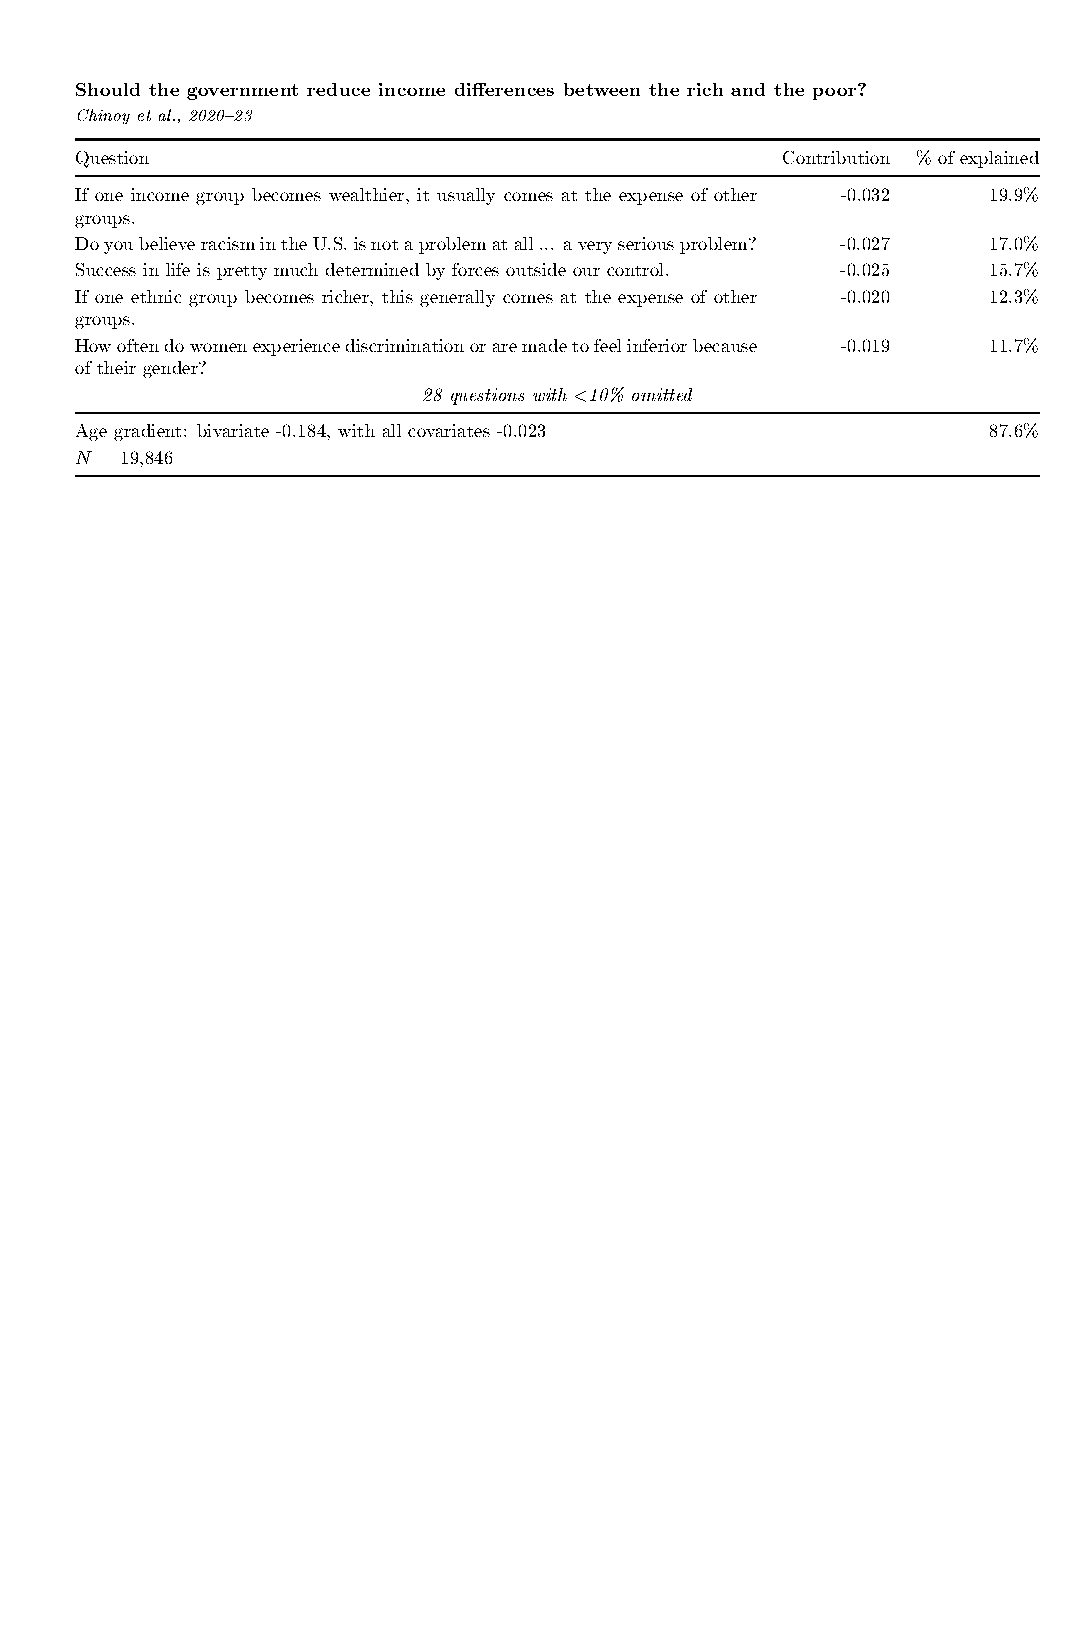
\includegraphics[width=0.9\linewidth]{figures/table_slide_gelbach_chinoy.pdf}
    \caption{Gelbach decomposition of \cite{chinoy2026zero}}
    \label{fig:placeholder}
\end{figure}
    
\end{frame}



\begin{frame}{Zero-sum or attribution beliefs?}

% Zero-sum wealth vs. attribution of unfair advantages and wealth extraction.
\begin{figure}
    \centering
    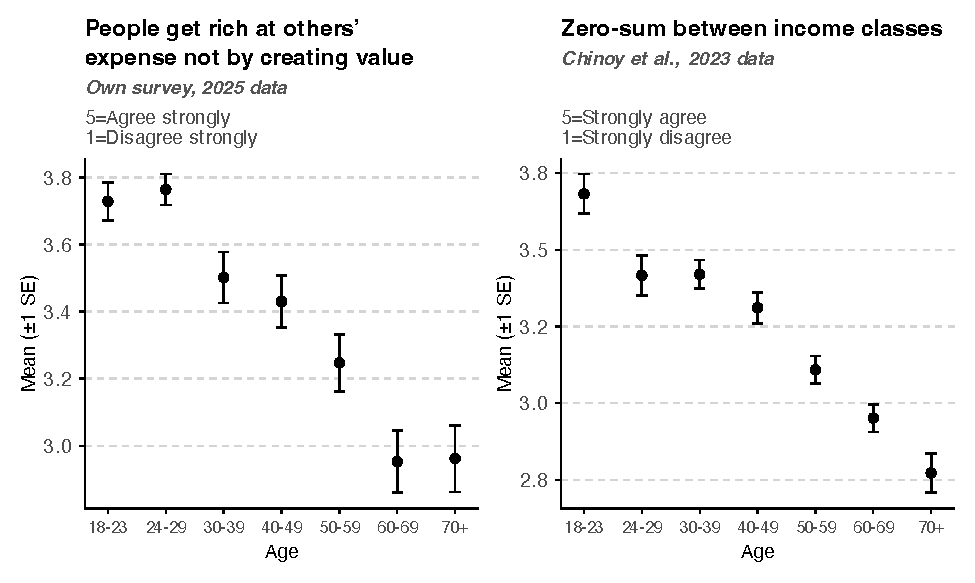
\includegraphics[width=0.9\linewidth]{figures/pair_zerosum_wealth.pdf}
    \caption{Recent age gradient in zero-sum income/wealth beliefs}
    \label{fig:placeholder}
\end{figure}
    
\end{frame}



\begin{frame}{Zero-sum or attribution beliefs?}

\begin{figure}
    \centering
    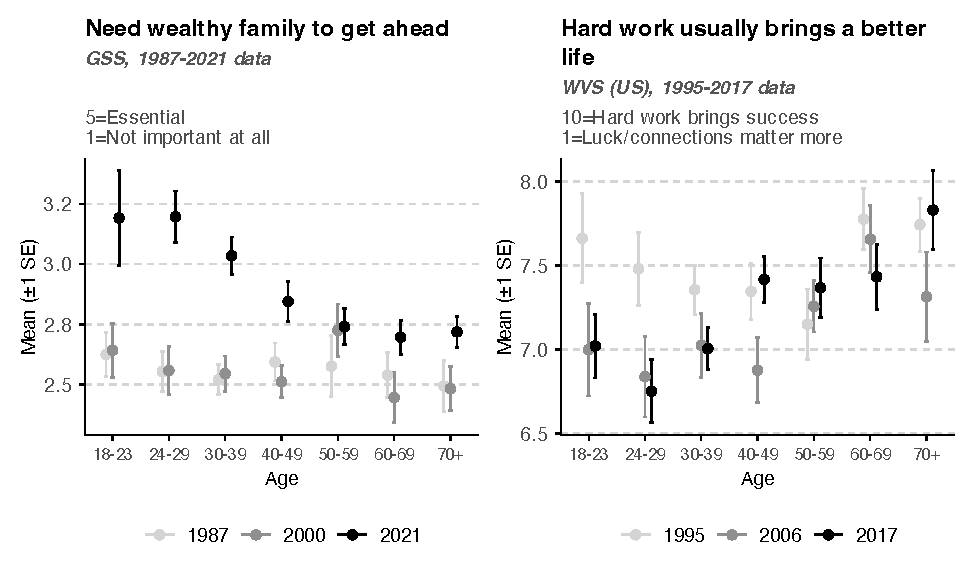
\includegraphics[width=0.9\linewidth]{figures/pair_attribution_wealth.pdf}
    \caption{Steepening age gradient in wealth attribution}
    \label{fig:placeholder}
\end{figure}
    
\end{frame}



\begin{frame}{Zero-sum or attribution beliefs?}

% Attribution of low effort and deservingness (racism).
\begin{figure}
    \centering
    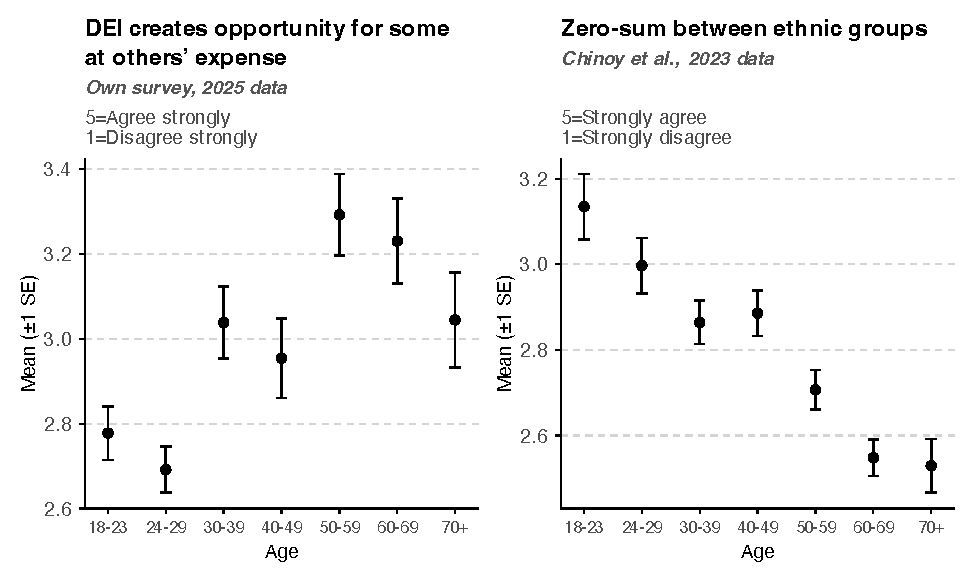
\includegraphics[width=0.9\linewidth]{figures/pair_zerosum_social.pdf}
    \caption{Recent age gradient in zero-sum social beliefs}
    \label{fig:placeholder}
\end{figure}
    
\end{frame}



\begin{frame}{Zero-sum or attribution beliefs?}

% Attribution of low effort and deservingness (racism).
\begin{figure}
    \centering
    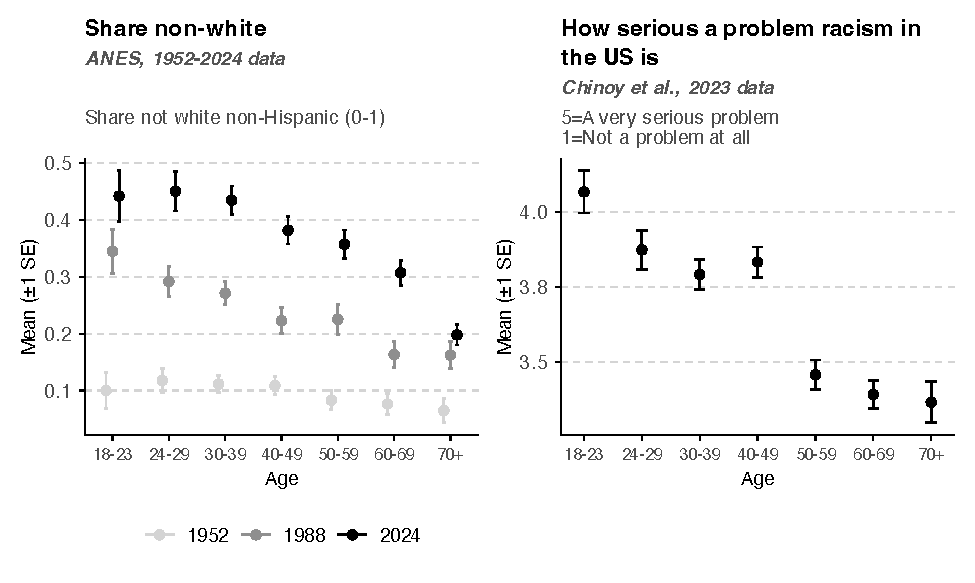
\includegraphics[width=0.9\linewidth]{figures/pair_attribution_race.pdf}
    \caption{Increasing diversity and diverging attitudes about race}
    \label{fig:placeholder}
\end{figure}
    
\end{frame}



\begin{frame}{Investigating belief drivers}

\begin{figure}
    \centering
    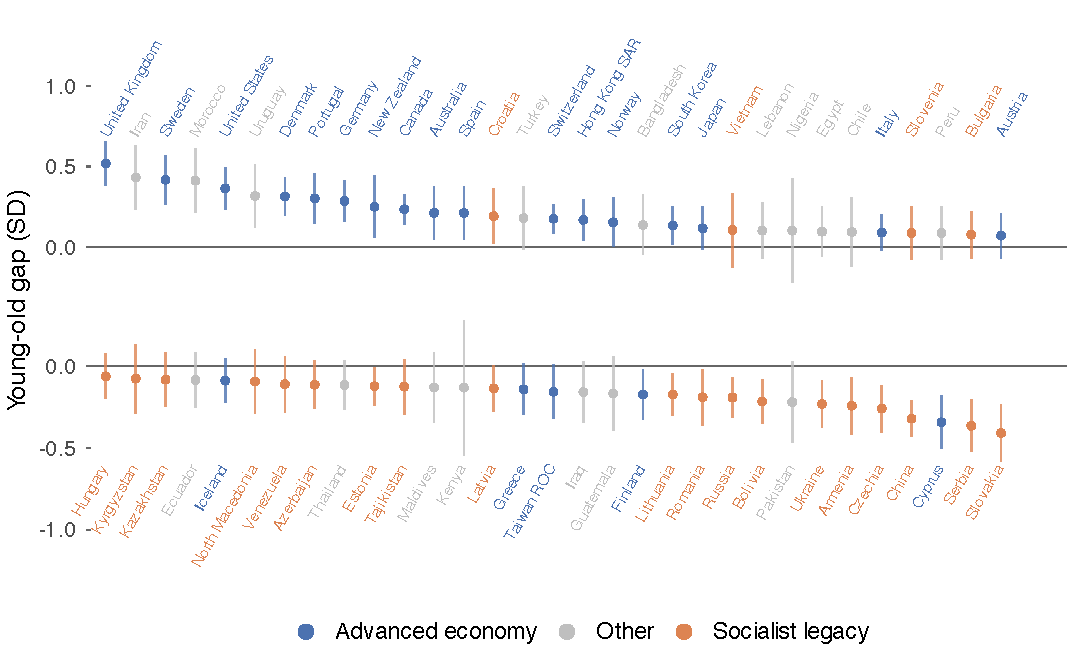
\includegraphics[width=0.85\linewidth]{figures/fig_slide_e037_ends.pdf}
    \caption{\centering Age gap in redistributive preferences in WVS/EVS wave 2017--2022, countries grouped by institutional history}
\end{figure}

\end{frame}



\begin{frame}{Investigating belief drivers}

\begin{figure}
    \centering
    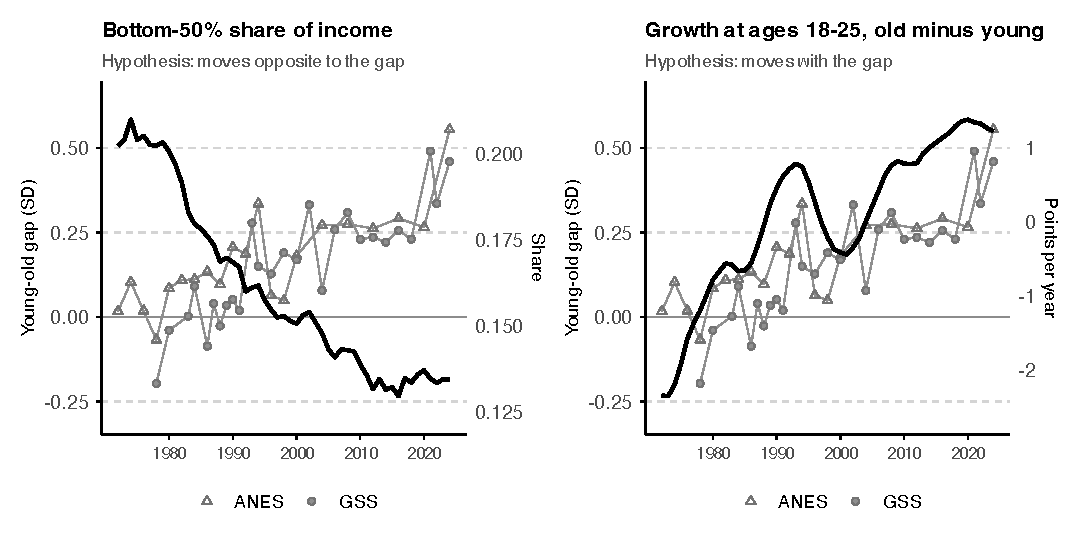
\includegraphics[width=0.9\linewidth]{figures/fig_slide_ts_pair.pdf}
    \caption{\centering Age gap in redistributive preferences versus current inequality and formative-years growth}
\end{figure}

\end{frame}



% \begin{frame}{Investigating drivers}

% Preliminary findings
% \begin{itemize}
%     \item Formative conditions alone do not explain it. Growth, inequality and mobility in a cohort's formative years predict at most 0.03 SD of a US gap of 0.3–0.7, and none of its rise. Chinoy's cross-country growth result does not replicate on our larger sample.
%     \item Institutional history does. On government responsibility, 11 of 28 advanced economies have a significant young-more-supportive gradient and 2 the reverse; in 33 countries with a socialist legacy it is 12 to 1 the other way. The US (−0.09) and UK (−0.12) are the steepest of 91.
% \end{itemize}

% \end{frame}



\begin{frame}{Investigating belief drivers}
% Investigating causality


Preliminary findings
\begin{itemize}
    \item Inequality, growth, and mobility alone do not explain any of the age gradient in cross-country analysis; the U.S. time series correlation is an outlier. 
    \item Trajectory of older Americans and non-formative-years placebo tests raise doubts about an imprinting story.
    \item Opposite age gradient on social security, emerging around 2020. 
    \item U.S. has highest perceived age conflict among rich democracies. Recently, the young perceive more conflict than the old.
    \item No age gap among Black Americans, only White/Hispanic.
    \item 3/4 of age gap survives within-party; not just higher polarization.
\end{itemize}
    
\end{frame}

\begin{frame}{Investigating belief drivers}

Why is the US unique? Possibilities:
\begin{itemize}
    \item Old-age benefits and the political power of the old
    \item Two-party bundling of cultural and economic positions (majoritarian vs. proportional system)
    \item Political entrepreneurs (Sanders, Trump)
    % Corbyn, Johnson. media narratives that place blame
    % Media segmentation: pre-2012 ANES access items show no differential gap; social-media batteries untested.
    % \item Social security and age representation in government
\end{itemize}
What explains sharp rise in gap post-2020?
\begin{itemize}
    \item Prominent billionaires reshaping society (Musk, Bezos)
    \item Racial justice salience (BLM movement)
    \item Affordability crisis (inflation, housing) and youth unemployment
    \item Government debt worries (social security more salient)
    \item Elderly presidential candidates in 2020 and 2024
\end{itemize}

\end{frame}

\begin{frame}{Investigating belief drivers}

Future analysis
\begin{itemize}
    \item Second survey wave
    \begin{itemize}
        \item A more comprehensive questionnaire pairing existing questions with govt. trust, religiosity, and race-related beliefs.
        \item In-depth measurement and differentiation of zero-sum/attribution beliefs. % which our current items partly confound
        \item An information provision or wording experiment generating exogenous belief variation.
    \end{itemize}
    \item Geographic and micro variation
    \begin{itemize}
        \item State and local-level age inequality measures: political representation (L2 voter files), policy tilt, real circumstances (housing, employment, etc.)
    \end{itemize}
    \item Text analysis
    \begin{itemize}
        \item Extracting zero-sum rich and zero-sum race narratives from Congressional speeches. Manifesto Project for cross-country.
    \end{itemize}
    % beliefs and preferences have moved a lot recently, so recent voter files (L2 and similar) and local exposure measures may give within-country variation.
\end{itemize}
    
\end{frame}



\begin{frame}[allowframebreaks]{References}

\bibliography{refs}

\nocite{alesina2018intergenerational}
\nocite{stantcheva2021understanding}


\end{frame}

\end{document}

